% !TeX program = xelatex
%─────────────────────────────────────────────────────────────────────────────
%  test_summary_20260417.tex
%  Beamer slide deck – 2026-04-17 업데이트: 유사도 버그 수정 후 재실험 결과
%─────────────────────────────────────────────────────────────────────────────
\documentclass[aspectratio=169,10pt]{beamer}

%─── 폰트 & 한국어 ───────────────────────────────────────────────────────────
\usepackage{fontspec}
\usepackage[hangul]{kotex}
\setmonofont{Consolas}

%─── 테마 ────────────────────────────────────────────────────────────────────
\usetheme{Madrid}
\usecolortheme{seahorse}
\usefonttheme[onlymath]{serif}
\setbeamertemplate{navigation symbols}{}
\setbeamertemplate{footline}{
	\leavevmode%
	\hbox{%
		\begin{beamercolorbox}[wd=.40\paperwidth,ht=2.25ex,dp=1ex,center]{author in head/foot}%
			\usebeamerfont{author in head/foot}\insertshortauthor
		\end{beamercolorbox}%
		\begin{beamercolorbox}[wd=.40\paperwidth,ht=2.25ex,dp=1ex,center]{title in head/foot}%
			\usebeamerfont{title in head/foot}\insertshorttitle
		\end{beamercolorbox}%
		\begin{beamercolorbox}[wd=.20\paperwidth,ht=2.25ex,dp=1ex,right]{date in head/foot}%
			\usebeamerfont{date in head/foot}
			\insertframenumber{} / \inserttotalframenumber\hspace*{2ex}
		\end{beamercolorbox}}%
	\vskip0pt%
}

%─── 패키지 ──────────────────────────────────────────────────────────────────
\usepackage{amsmath,amssymb,bm}
\usepackage{booktabs}
\usepackage{colortbl}
\usepackage{xcolor}
\usepackage{tikz}
\usetikzlibrary{positioning,arrows,decorations.pathreplacing}
\usepackage{graphicx}

%─── 색 정의 ─────────────────────────────────────────────────────────────────
\definecolor{posblue}{RGB}{30,100,200}
\definecolor{negred}{RGB}{210,40,40}
\definecolor{testgreen}{RGB}{0,150,80}
\definecolor{hilight}{RGB}{255,230,100}

%─── 메타정보 ─────────────────────────────────────────────────────────────────
\title[버그 수정 후 재실험 결과]{유사도 구현 버그 수정 후 재실험 결과\\
			 \small \texttt{msd} / \texttt{jmsd} / \texttt{acos} --- $\lambda=0$, 10-Fold 전체}
\subtitle{2026-04-17 업데이트 -- \texttt{similarities.py} 버그 수정 결과 분석}
\author[발표자]{[]}
\institute{[]}
\date{2026년 4월 17일}

\begin{document}

%─────────────────────────────────────────────────────────────────────────────
\begin{frame}
	\titlepage
\end{frame}

\begin{frame}{목차}
	\tableofcontents[hideallsubsections]
\end{frame}

%═════════════════════════════════════════════════════════════════════════════
\section{버그 수정 후 재실험 결과 분석 ($\lambda=0$)}
%═════════════════════════════════════════════════════════════════════════════

%── 책갈피 ────────────────────────────────────────────────────────────────────
\begin{frame}[plain]
	\begin{center}
		\vspace{1.8cm}
		{\LARGE \textbf{2026-04-17 업데이트}}\\[0.8em]
		{\large \texttt{similarities.py} 버그 수정 + 재실험 완료}\\[0.6em]
		{\normalsize 영향 범위: \texttt{msd} / \texttt{jmsd} / \texttt{acos} --- $\lambda=0$, 10-Fold 전체 재실험}\\[1em]
		{\small \textcolor{negred}{분석 방법: 버기 $\lambda=0$ vs 수정 후 $\lambda=0$ (순수 버그 효과 비교)}}
	\end{center}
\end{frame}

%── 슬라이드 1: 버그 요약 ─────────────────────────────────────────────────────
\begin{frame}[shrink=8]{버그 수정 요약 및 재실험 조건}
	\begin{columns}[T]
		\column{0.54\textwidth}
			\renewcommand{\arraystretch}{1.3}
			\begin{tabular}{l|p{3.4cm}|p{2.8cm}}
				\toprule
				\textbf{메서드} & \textbf{버그 → 수정} & \textbf{영향} \\
				\midrule
				\texttt{msd}
				  & $\tfrac{x}{5}-\tfrac{y}{5}$ $\to$ $\tfrac{x-y}{4}$
				  & 범위 $[0.36,1]$$\to$$[0,1]$ \\
				\texttt{jmsd}
				  & \texttt{msd()} 호출 상속
				  & msd 와 동일 \\
				\texttt{acos}
				  & user-mean $\to$ item-mean
				  & 범위 $\approx\!0$ $\to$ $[-1,+1]$ \\
				\bottomrule
			\end{tabular}

			\vspace{0.4em}
			\begin{block}{비교 방법론 (수정)}
				\small
				\textbf{올바른 비교}: 버기 $\lambda=0$ \ vs \ 수정 $\lambda=0$\\
				\textcolor{negred}{$\times$ 잘못된 비교}: 버기 $\lambda=0.002$ vs 수정 $\lambda=0$\\
				\small → $\lambda$ 변경 효과($\approx-0.002$)가 혼재되므로 제외
			\end{block}

		\column{0.43\textwidth}
			\begin{alertblock}{재실험 조건}
				\begin{itemize}
					\item $\lambda = 0$, 10-fold 전체 (558분)
					\item msd / jmsd / acos 3개 재실험
					\item 나머지 14개 기존 결과 재사용
				\end{itemize}
			\end{alertblock}
			\begin{block}{결론 선요약}
				\small
				\textbf{acos}: Δ$\approx-0.06$ (버그 영향 최대)\\
				\textbf{jmsd}: Δ$\approx-0.005$$\sim$$-0.007$\\
				\textbf{msd}: Δ$\approx$0$\sim$$-0.005$ (효과 제한적)\\
				\small \textcolor{negred}{MSD K=10 α*: 9.95→7.2 정상화됨}
			\end{block}
	\end{columns}
\end{frame}

%── 슬라이드 2: MSD before/after ─────────────────────────────────────────────
\begin{frame}[shrink=20]{수정 전·후 비교: \texttt{msd} \textnormal{\small(버기 $\lambda=0$ vs 수정 $\lambda=0$, 10-fold 평균)}}
	\begin{columns}[T]
		\column{0.55\textwidth}
		\begin{center}
		\renewcommand{\arraystretch}{1.15}
		\small
		\begin{tabular}{c|cc|cc|r}
			\toprule
			& \multicolumn{2}{c|}{\textbf{버기} ($\lambda=0$)} & \multicolumn{2}{c|}{\textbf{수정} ($\lambda=0$)} & \\
			$K$ & $\alpha^*_b$ & RMSE$_b$ & $\alpha^*_f$ & RMSE$_f$ & $\Delta$ RMSE \\
			\midrule
			\rowcolor{hilight!40}
			10  &  9.950 & 0.9868 &  7.200 & 0.9867 & $\approx$0 \\
			20  & 10.000 & 0.9727 & 10.000 & 0.9719 & \textcolor{testgreen}{$-$0.0008 $\downarrow$} \\
			30  & 10.000 & 0.9721 & 10.000 & 0.9704 & \textcolor{testgreen}{$-$0.0017 $\downarrow$} \\
			40  & 10.000 & 0.9735 & 10.000 & 0.9710 & \textcolor{testgreen}{$-$0.0025 $\downarrow$} \\
			50  & 10.000 & 0.9753 & 10.000 & 0.9722 & \textcolor{testgreen}{$-$0.0031 $\downarrow$} \\
			60  & 10.000 & 0.9773 & 10.000 & 0.9737 & \textcolor{testgreen}{$-$0.0037 $\downarrow$} \\
			70  & 10.000 & 0.9792 & 10.000 & 0.9751 & \textcolor{testgreen}{$-$0.0042 $\downarrow$} \\
			80  & 10.000 & 0.9811 & 10.000 & 0.9765 & \textcolor{testgreen}{$-$0.0046 $\downarrow$} \\
			90  & 10.000 & 0.9828 & 10.000 & 0.9778 & \textcolor{testgreen}{$-$0.0050 $\downarrow$} \\
			100 & 10.000 & 0.9843 & 10.000 & 0.9789 & \textcolor{testgreen}{$-$0.0054 $\downarrow$} \\
			\bottomrule
		\end{tabular}
		\end{center}

		\column{0.43\textwidth}
			\begin{alertblock}{핵심 발견: K=10 ($\alpha^*$ 정상화)}
				\small
				\textbf{버기 λ=0}: K=10의 $\alpha^*=9.95$ (그리드 상한 근접)\\
				\textbf{수정 후}: K=10의 $\alpha^*=7.2$ → \textbf{자연 수렴!}\\
				\vspace{0.3em}
				버그가 K=10에서도 $\alpha$를 그리드 상한으로 끌어올렸음이 증명됨.\\
				RMSE 변화는 K=10에서 $\approx 0$ (무변화)
			\end{alertblock}
			\begin{block}{K$\geq$20 해석}
				\small
				버기·수정 모두 $\alpha^*=10.0$ (상한 고착)\\
				→ 버그와 무관한 \textbf{msd 유사도 분포 특성}\\
				(83.8\%가 $\geq 0.8$, 강한 집중 분포)\\
				RMSE 개선 $\Delta\approx-0.001$$\sim$$-0.005$\\
				\textcolor{negred}{그리드 상한 확장 ($\leq 30$) 필요}
			\end{block}
	\end{columns}
\end{frame}

%── 슬라이드 3: JMSD before/after ────────────────────────────────────────────
\begin{frame}[shrink=20]{수정 전·후 비교: \texttt{jmsd} \textnormal{\small(버기 $\lambda=0$ vs 수정 $\lambda=0$, 10-fold 평균)}}
	\begin{columns}[T]
		\column{0.55\textwidth}
		\begin{center}
		\renewcommand{\arraystretch}{1.15}
		\small
		\begin{tabular}{c|cc|cc|r}
			\toprule
			& \multicolumn{2}{c|}{\textbf{버기} ($\lambda=0$)} & \multicolumn{2}{c|}{\textbf{수정} ($\lambda=0$)} & \\
			$K$ & $\alpha^*_b$ & RMSE$_b$ & $\alpha^*_f$ & RMSE$_f$ & $\Delta$ RMSE \\
			\midrule
			10  & 1.110 & 1.0165 & 1.255 & 1.0096 & \textcolor{testgreen}{$-$0.0070 $\downarrow$} \\
			20  & 1.400 & 1.0047 & 1.675 & 0.9983 & \textcolor{testgreen}{$-$0.0064 $\downarrow$} \\
			30  & 1.665 & 1.0029 & 1.950 & 0.9972 & \textcolor{testgreen}{$-$0.0057 $\downarrow$} \\
			40  & 1.850 & 1.0033 & 2.155 & 0.9979 & \textcolor{testgreen}{$-$0.0054 $\downarrow$} \\
			50  & 1.990 & 1.0039 & 2.325 & 0.9988 & \textcolor{testgreen}{$-$0.0051 $\downarrow$} \\
			60  & 2.110 & 1.0044 & 2.445 & 0.9995 & \textcolor{testgreen}{$-$0.0049 $\downarrow$} \\
			70  & 2.215 & 1.0050 & 2.530 & 1.0002 & \textcolor{testgreen}{$-$0.0049 $\downarrow$} \\
			80  & 2.275 & 1.0055 & 2.625 & 1.0007 & \textcolor{testgreen}{$-$0.0048 $\downarrow$} \\
			90  & 2.355 & 1.0059 & 2.690 & 1.0011 & \textcolor{testgreen}{$-$0.0048 $\downarrow$} \\
			100 & 2.405 & 1.0063 & 2.740 & 1.0015 & \textcolor{testgreen}{$-$0.0048 $\downarrow$} \\
			\bottomrule
		\end{tabular}
		\end{center}

		\column{0.42\textwidth}
			\begin{block}{$\alpha^*$ 변화}
				\small
				jmsd = Jaccard $\times$ msd 구조.\\msd 수정이 그대로 전파됨.\\
				$\alpha^*$ 전반적으로 \textbf{+0.1$\sim$+0.3} 상승.\\
				K 증가에 따라 $\alpha^*$ 단조 증가 패턴 유지.\\
				alpha 그리드 상한에 걸리지 않음 (최대 2.74)
			\end{block}
			\begin{alertblock}{RMSE 개선}
				\small
				K=10: $\Delta=-0.0070$\\
				K=20$\sim$100: $\Delta\approx-0.005$$\sim-0.006$\\
				전 K에서 균등하고 일관된 개선.\\
				msd보다 개선 폭 크고 안정적.
			\end{alertblock}
	\end{columns}
\end{frame}

%── 슬라이드 4: ACOS before/after ────────────────────────────────────────────
\begin{frame}[shrink=20]{수정 전·후 비교: \texttt{acos} \textnormal{\small(버기 $\lambda=0$ vs 수정 $\lambda=0$, 10-fold 평균)}}
	\begin{columns}[T]
		\column{0.55\textwidth}
		\begin{center}
		\renewcommand{\arraystretch}{1.15}
		\small
		\begin{tabular}{c|cc|cc|r}
			\toprule
			& \multicolumn{2}{c|}{\textbf{버기} ($\lambda=0$)} & \multicolumn{2}{c|}{\textbf{수정} ($\lambda=0$)} & \\
			$K$ & $\alpha^*_b$ & RMSE$_b$ & $\alpha^*_f$ & RMSE$_f$ & $\Delta$ RMSE \\
			\midrule
			\rowcolor{negred!15}
			10  & 6.800 & 1.0412 & 0.180 & 0.9766 & \textcolor{testgreen}{$-$0.0646 $\downarrow$} \\
			20  & 0.050 & 1.0192 & 0.340 & 0.9583 & \textcolor{testgreen}{$-$0.0609 $\downarrow$} \\
			30  & 0.050 & 1.0129 & 0.435 & 0.9549 & \textcolor{testgreen}{$-$0.0580 $\downarrow$} \\
			40  & 0.050 & 1.0108 & 0.505 & 0.9541 & \textcolor{testgreen}{$-$0.0567 $\downarrow$} \\
			50  & 0.055 & 1.0100 & 0.555 & 0.9541 & \textcolor{testgreen}{$-$0.0559 $\downarrow$} \\
			60  & 0.060 & 1.0100 & 0.585 & 0.9543 & \textcolor{testgreen}{$-$0.0557 $\downarrow$} \\
			70  & 0.070 & 1.0105 & 0.615 & 0.9547 & \textcolor{testgreen}{$-$0.0557 $\downarrow$} \\
			80  & 0.080 & 1.0108 & 0.635 & 0.9550 & \textcolor{testgreen}{$-$0.0557 $\downarrow$} \\
			90  & 0.100 & 1.0112 & 0.640 & 0.9553 & \textcolor{testgreen}{$-$0.0558 $\downarrow$} \\
			100 & 0.105 & 1.0116 & 0.660 & 0.9555 & \textcolor{testgreen}{$-$0.0562 $\downarrow$} \\
			\bottomrule
		\end{tabular}
		\end{center}

		\column{0.42\textwidth}
			\begin{alertblock}{K=10 이상치 해소}
				\small
				\textbf{버기}: K=10만 $\alpha^*=6.8$, K$\geq$20에서 $\alpha^*\approx0.05$ (이분화)\\
				item-mean centering 누락으로 유사도$\approx 0$ 근방 압축\\
				\vspace{0.3em}
				\textbf{수정 후}: $\alpha^*=0.18$$\sim$$0.66$, \textbf{단조 증가}, 이상치 완전 해소
			\end{alertblock}
			\begin{exampleblock}{수정 효과 — 3메서드 중 최대}
				\small
				$\Delta$RMSE $\approx -0.056$$\sim$$-0.065$ (전 K)\\
				RMSE 0.95$\sim$0.98대 진입 (수정 전: 1.01$\sim$1.04)\\
				\textbf{수정 후 전체 1위 메서드로 부상}
			\end{exampleblock}
	\end{columns}
\end{frame}

%── 슬라이드 5: MSD Alpha 포화 분석 ──────────────────────────────────────────
\begin{frame}[shrink=10]{MSD $\alpha^*$ 그리드 상한 포화: 버그 vs 고유 특성 구분}
	\begin{columns}[T]
		\column{0.49\textwidth}
			\begin{alertblock}{버기 vs 수정: K=10 비교}
				\small
				\begin{tabular}{l|cc}
					\toprule
					버전 & K=10 $\alpha^*$ & K$\geq$20 $\alpha^*$ \\
					\midrule
					버기 ($\lambda=0$) & 9.95 (상한 근접!) & 10.0 (상한) \\
					수정 ($\lambda=0$) & 7.2 (\textbf{정상 수렴}) & 10.0 (상한) \\
					\bottomrule
				\end{tabular}
				\vspace{0.3em}
				\small K=10: 버그 영향으로 과도 상승 → 수정 후 자연 수렴.\\K$\geq$20: 버기/수정 모두 상한 → \textbf{msd 고유 특성}
			\end{alertblock}

			\begin{block}{msd 유사도 분포 (fold\_01, 수정 후)}
				\small
				\begin{tabular}{l|rrc}
					\toprule
					메서드 & mean & std & $\geq 0.8$ 비율 \\
					\midrule
					msd  & 0.872 & 0.096 & 83.8\% \\
					jmsd & 0.063 & 0.043 & $\approx$0\% \\
					acos & 0.374 & 0.281 & — \\
					\bottomrule
				\end{tabular}
			\end{block}

		\column{0.49\textwidth}
			\begin{block}{$S^\alpha$ 변환: $\alpha$ 크기에 따른 이웃 구별력}
				\small
				\begin{tabular}{r|r|r}
					\toprule
					$\alpha$ & p75/p25 비 & 구별력 \\
					\midrule
					1.0  & 1.12$\times$ & 낮음 \\
					5.0  & 1.74$\times$ & 중간 \\
					10.0 & 3.02$\times$ & 높음 (상한) \\
					20.0 & 9.15$\times$ & 매우 높음 \\
					\bottomrule
				\end{tabular}
				\vspace{0.2em}
				\small msd가 $[0.8, 1.0]$에 밀집 → $\alpha=1$로는 이웃 간 차이 미미.\\높은 $\alpha$로 가중치 집중이 필요.
			\end{block}
			\begin{exampleblock}{결론 및 권고}
				\small
				K$\geq$20의 $\alpha^*=10$ 고착: 버그와 무관, \textbf{msd 분포 고유 특성}.\\
				$\alpha=10$에서도 RMSE 여전히 감소 중 → 진정한 최적값은 10 이상.\\
				\textbf{권고}: 그리드 상한 $10 \to 30$ 확장 필요.
			\end{exampleblock}
	\end{columns}
\end{frame}

%── 슬라이드 6: 17개 메서드 최종 순위 비교 ───────────────────────────────────
\begin{frame}[shrink=8]{17개 메서드 최종 순위: 수정 전·후 비교 \textnormal{\small($\lambda=0$, 10-fold 평균, Opt RMSE)}}
	\begin{columns}[T]
		\column{0.50\textwidth}
			\begin{block}{수정 \textbf{전} (버기 결과, All-$K$ 평균 기준)}
				\renewcommand{\arraystretch}{1.1}
				\scriptsize
				\begin{tabular}{r|l|r}
					\toprule
					순위 & 메서드 & RMSE \\
					\midrule
					1 & ipwr     & 0.9716 \\
					2 & msd\quad\textcolor{negred}{★} & 0.9785 \\
					3 & cpcc     & 0.9872 \\
					4 & chebyshev & 1.0044 \\
					5 & jmsd\quad\textcolor{negred}{★} & 1.0058 \\
					6 & spcc     & 1.0075 \\
					7 & pcc      & 1.0084 \\
					8 & euclidean & 1.0100 \\
					9 & cosine   & 1.0102 \\
					10 & src     & 1.0128 \\
					11 & kendall\_tau\_b & 1.0129 \\
					\rowcolor{negred!15}
					12 & \textbf{acos}\quad\textcolor{negred}{★} & \textbf{1.0148} \\
					13 & jaccard  & 1.0152 \\
					14 & manhattan & 1.0180 \\
					15 & itr      & 1.0255 \\
					16 & ari      & 1.0262 \\
					17 & ami      & 1.0285 \\
					\bottomrule
				\end{tabular}
				\vspace{0.2em}
				{\tiny acos 12위, msd 2위, jmsd 5위}
			\end{block}

		\column{0.48\textwidth}
			\begin{alertblock}{수정 \textbf{후} (10-fold, All-$K$ 평균 기준)}
				\renewcommand{\arraystretch}{1.1}
				\scriptsize
				\begin{tabular}{r|l|r}
					\toprule
					순위 & 메서드 & RMSE \\
					\midrule
					\rowcolor{testgreen!25}
					\textbf{1} & \textbf{acos\quad\textcolor{testgreen}{★}} & \textbf{0.9573} \\
					2 & ipwr     & 0.9717 \\
					\rowcolor{testgreen!10}
					3 & msd\quad\textcolor{testgreen}{★} & 0.9754 \\
					4 & cpcc     & 0.9872 \\
					\rowcolor{testgreen!10}
					5 & jmsd\quad\textcolor{testgreen}{★} & 1.0005 \\
					6 & chebyshev & 1.0046 \\
					7 & spcc     & 1.0076 \\
					8 & pcc      & 1.0085 \\
					9 & euclidean & 1.0100 \\
					10 & cosine  & 1.0105 \\
					11 & src     & 1.0127 \\
					12 & kendall\_tau\_b & 1.0129 \\
					13 & jaccard & 1.0153 \\
					14 & manhattan & 1.0181 \\
					15 & itr     & 1.0258 \\
					16 & ari     & 1.0262 \\
					17 & ami     & 1.0284 \\
					\bottomrule
				\end{tabular}
				\vspace{0.2em}
				{\tiny ★수정됨 (msd/jmsd/acos). 수정 후: All-$K$ 평균 방식 적용.}
			\end{alertblock}
	\end{columns}
\end{frame}

%── 슬라이드 7: Alpha 선택 분포 수정 후 ─────────────────────────────────────
\begin{frame}[shrink=25]{수정 후 $\alpha^*$ 선택 분포: msd / jmsd / acos \textnormal{\small(10-fold 평균, all TopN 평균)}}
	\begin{center}
	\renewcommand{\arraystretch}{1.2}
	\small
	\begin{tabular}{l|rrrrrrrrrr|rrr}
		\toprule
		Method & K=10 & K=20 & K=30 & K=40 & K=50 & K=60 & K=70 & K=80 & K=90 & K=100 & Mean & Std & Max \\
		\midrule
		\textbf{msd (수정 후)}
		  & 7.200 & 10.000 & 10.000 & 10.000 & 10.000 & 10.000 & 10.000 & 10.000 & 10.000 & 10.000
		  & 9.720 & 0.854 & 10.0 \\
		\textbf{msd (버기 $\lambda=0$)}
		  & 9.950 & 10.000 & 10.000 & 10.000 & 10.000 & 10.000 & 10.000 & 10.000 & 10.000 & 10.000
		  & 9.995 & 0.158 & 10.0 \\
		\midrule
		\textbf{jmsd (수정 후)}
		  & 1.255 & 1.675 & 1.950 & 2.155 & 2.325 & 2.445 & 2.530 & 2.625 & 2.690 & 2.740
		  & 2.239 & 0.484 & 2.74 \\
		\textbf{jmsd (버기 $\lambda=0$)}
		  & 1.110 & 1.400 & 1.665 & 1.850 & 1.990 & 2.110 & 2.215 & 2.275 & 2.355 & 2.405
		  & 1.938 & 0.439 & 2.41 \\
		\midrule
		\textbf{acos (수정 후)}
		  & 0.180 & 0.340 & 0.435 & 0.505 & 0.555 & 0.585 & 0.615 & 0.635 & 0.640 & 0.660
		  & 0.515 & 0.153 & 0.66 \\
		\textbf{acos (버기 $\lambda=0$)}
		  & 6.800 & 0.050 & 0.050 & 0.050 & 0.055 & 0.060 & 0.070 & 0.080 & 0.100 & 0.105
		  & 0.742 & 2.075 & 6.80 \\
		\bottomrule
	\end{tabular}
	\end{center}

	\vspace{0.3em}
	\begin{columns}[T]
		\column{0.48\textwidth}
			\begin{block}{msd $\alpha^*$ 변화}
				\small
				버기($\lambda=0$): K=10{\,}=9.95 (상한 근접), K$\geq$20 모두 10.0 (상한 고착).\\
				수정 후: K=10만 7.2로 자연 수렴, K$\geq$20 여전히 10.0 → msd 고유 특성.
			\end{block}
		\column{0.48\textwidth}
			\begin{alertblock}{acos $\alpha^*$ 이상치 해소}
				버기 K=10: $\alpha^*=6.778$ (이상치), K$\geq$20: $\alpha^*\approx0.05$ (이분화) \\
				수정 후: 0.18$\sim$0.66으로 \textbf{단조 증가}, std=0.153으로 안정화
			\end{alertblock}
	\end{columns}
\end{frame}

%── 슬라이드 8: 종합 결론 ─────────────────────────────────────────────────────
\begin{frame}[shrink=15]{종합 결론: 버그 수정 순수 효과 분석 (올바른 비교 기준)}
	\begin{columns}[T]
		\column{0.50\textwidth}
			\begin{alertblock}{3개 메서드 버그 수정 순수 효과}
				\small
				\renewcommand{\arraystretch}{1.15}
				\begin{tabular}{l|r|l}
					\toprule
					메서드 & $\Delta$RMSE (대표) & 주요 변화 \\
					\midrule
					\textbf{acos}  & $-0.056$$\sim$$-0.065$ & \textbf{최대 개선} \\
					\textbf{jmsd}  & $-0.005$$\sim$$-0.007$ & 균등 개선 \\
					\textbf{msd}   & $\approx 0$$\sim$$-0.005$ & 제한적 \\
					\bottomrule
				\end{tabular}
			\end{alertblock}
			\begin{block}{MSD 핵심 발견 (재분석)}
				\small
				\begin{itemize}
					\item 버기에서도 K=10 $\alpha^*=9.95$ (상한 근접): 버그가 K=10까지 영향
					\item 수정 후 K=10 $\alpha^*=7.2$: 자연 수렴 확인
					\item K$\geq$20: 버기·수정 모두 $\alpha^*=10$ → \textbf{msd 고유 특성}
					\item RMSE 개선: K=10$\approx 0$, K$\geq$20 $\approx -0.001$$\sim$$-0.005$
				\end{itemize}
			\end{block}

		\column{0.47\textwidth}
			\begin{exampleblock}{17개 메서드 최종 순위 (수정 후, All-$K$ 평균)}
				\small
				\textbf{1위 acos} (0.9573) \textcolor{testgreen}{★}\\
				2위 ipwr (0.9717)\\
				\textbf{3위 msd} (0.9754) \textcolor{testgreen}{★}\\
				4위 cpcc (0.9872)\\
				\textbf{5위 jmsd} (1.0005) \textcolor{testgreen}{★}\\
				{\tiny ★: 이번 버그 수정 대상. All-$K$ 평균 기준.}
			\end{exampleblock}
			\begin{block}{후속 권고}
				\small
				\begin{itemize}
					\item msd: $\alpha$ 그리드 상한 $10 \to 30$ 확장 $\Rightarrow$ K$\geq$20 진정한 최적 $\alpha$ 탐색
					\item acos: item-mean centering이 가장 중요한 수정 사항. 논문에 명시 필요.
					\item 논문 수치: 수정된 $\lambda=0$ 기반으로 전면 교체
				\end{itemize}
			\end{block}
	\end{columns}
\end{frame}

%═════════════════════════════════════════════════════════════════════════════
\appendix
%═════════════════════════════════════════════════════════════════════════════

\begin{frame}[shrink=20]{Appendix: 수정된 핵심 수식}
	\begin{columns}[T]
		\column{0.48\textwidth}
			\textbf{\texttt{msd} 수정}
			\begin{exampleblock}{수정 후}
				\[ \text{MSD}(u,v) = 1 - \frac{\displaystyle\sum_{i\in I_{uv}}\!\left(\tfrac{x_i-y_i}{4}\right)^2}{|I_{uv}|} \]
			\end{exampleblock}
		\column{0.48\textwidth}
			\textbf{\texttt{acos} 수정}
			\begin{exampleblock}{수정 후 (item-mean centering)}
				\[ \text{ACOS}(u,v) = \frac{\displaystyle\sum_{i\in I_{uv}}(x_i-\bar{r}_i)(y_i-\bar{r}_i)}{\sqrt{\cdots}\,\sqrt{\cdots}} \]
				{\small $\bar{r}_i = \frac{1}{|\mathcal{U}_i|}\sum_u r_{ui}$: 아이템 평균 평점}
			\end{exampleblock}
	\end{columns}

	\vspace{0.5em}
	\begin{block}{$\alpha$ 지수 변환}
		\[ S_{uv}^{(\alpha)} = \max(S_{uv},0)^{\alpha}, \qquad
		   \hat{r}_{ui} = \frac{\displaystyle\sum_{v\in\mathcal{N}_K(u,i)} S_{uv}^{(\alpha)}r_{vi}}
		                       {\displaystyle\sum_{v\in\mathcal{N}_K(u,i)} S_{uv}^{(\alpha)}} \]
	\end{block}
\end{frame}

%─────────────────────────────────────────────────────────────────────────────
\begin{frame}[shrink=10]{MSD: Fold별 최적 $\alpha^*$ 선택값 --- $K=10$}
	\framesubtitle{버기(Buggy) vs.\ 수정(Fixed) 비교}

	\begin{columns}[T]
		\column{0.52\textwidth}
			\centering
			\small
			\begin{tabular}{ccc}
				\toprule
				\textbf{Fold} & \textbf{Buggy $\alpha^*$} & \textbf{Fixed $\alpha^*$} \\
				\midrule
				1  & 1.0 & \cellcolor{posblue!25}8.5 \\
				2  & 1.0 & \cellcolor{posblue!25}7.5 \\
				3  & 1.0 & \cellcolor{posblue!25}6.5 \\
				4  & 1.0 & \cellcolor{posblue!25}8.5 \\
				5  & 1.0 & \cellcolor{posblue!25}6.5 \\
				6  & 1.0 & \cellcolor{posblue!25}7.0 \\
				7  & 1.0 & \cellcolor{posblue!25}6.0 \\
				8  & 1.0 & \cellcolor{posblue!25}7.5 \\
				9  & 1.0 & \cellcolor{posblue!25}6.0 \\
				10 & 1.0 & \cellcolor{posblue!25}8.0 \\
				\midrule
				\textbf{평균} & \textbf{1.00} & \cellcolor{posblue!40}\textbf{7.25} \\
				\bottomrule
			\end{tabular}

		\column{0.48\textwidth}
			\centering
			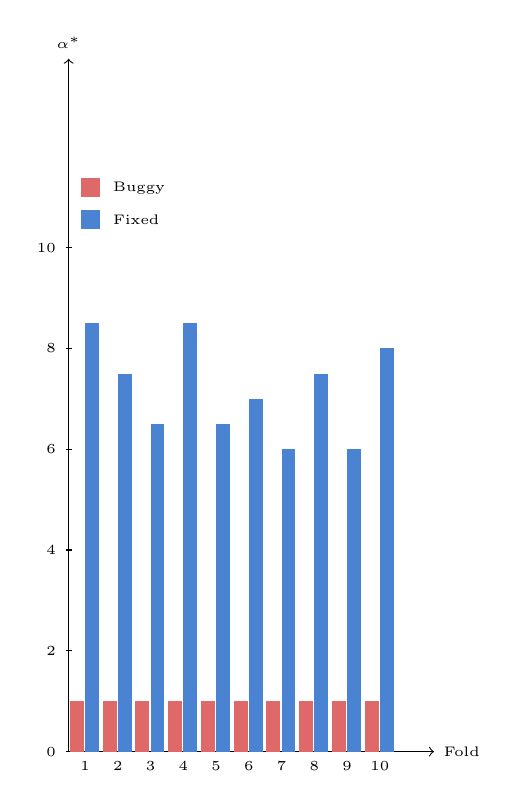
\begin{tikzpicture}[scale=0.80]
				\pgfmathsetmacro{\ymax}{11}
				% axes
				\draw[->] (0,0) -- (0,\ymax) node[above,font=\tiny]{$\alpha^*$};
				\draw[->] (0,0) -- (5.8,0) node[right,font=\tiny]{Fold};
				% y ticks
				\foreach \y in {0,2,4,6,8,10}{
					\draw (-0.05,\y*0.8) -- (0.05,\y*0.8);
					\node[left,font=\tiny] at (-0.05,\y*0.8) {\y};
				}
				% x ticks
				\foreach \i/\lbl in {1/1,2/2,3/3,4/4,5/5,6/6,7/7,8/8,9/9,10/10}{
					\pgfmathsetmacro{\xpos}{(\i-0.5)*0.52}
					\node[below,font=\tiny] at (\xpos,0) {\lbl};
				}
				% Buggy bars (all 1.0) -- red
				\foreach \i/\val in {1/1.0,2/1.0,3/1.0,4/1.0,5/1.0,6/1.0,7/1.0,8/1.0,9/1.0,10/1.0}{
					\pgfmathsetmacro{\xpos}{(\i-1)*0.52+0.02}
					\pgfmathsetmacro{\h}{\val*0.8}
					\fill[negred!70] (\xpos,0) rectangle ++(0.22,\h);
				}
				% Fixed bars -- blue
				\foreach \i/\val in {1/8.5,2/7.5,3/6.5,4/8.5,5/6.5,6/7.0,7/6.0,8/7.5,9/6.0,10/8.0}{
					\pgfmathsetmacro{\xpos}{(\i-1)*0.52+0.26}
					\pgfmathsetmacro{\h}{\val*0.8}
					\fill[posblue!80] (\xpos,0) rectangle ++(0.22,\h);
				}
				% legend
				\fill[negred!70] (0.2,8.8) rectangle ++(0.3,0.3);
				\node[right,font=\tiny] at (0.55,8.95) {Buggy};
				\fill[posblue!80] (0.2,8.3) rectangle ++(0.3,0.3);
				\node[right,font=\tiny] at (0.55,8.45) {Fixed};
			\end{tikzpicture}

			\vspace{0.3em}
			{\small\color{negred}$\Rightarrow$ 버그 버전: 유사도 범위 $[0.36,1]$로 압축 $\rightarrow$ $\alpha$ 변환 효과 미미 $\rightarrow$ $\alpha^*=1.0$}\\[2pt]
			{\small\color{posblue}$\Rightarrow$ 수정 후: 유사도 범위 $[0,1]$ 정상화 $\rightarrow$ $\alpha^* \in [6.0,\,8.5]$ (fold마다 다른 지역 최적값)}
	\end{columns}
\end{frame}

%─────────────────────────────────────────────────────────────────────────────
\begin{frame}[shrink=10]{MSD: Fold별 최적 $\alpha^*$ 선택값 --- $K=20$}
	\framesubtitle{버기(Buggy) vs.\ 수정(Fixed) 비교}

	\begin{columns}[T]
		\column{0.52\textwidth}
			\centering
			\small
			\begin{tabular}{ccc}
				\toprule
				\textbf{Fold} & \textbf{Buggy $\alpha^*$} & \textbf{Fixed $\alpha^*$} \\
				\midrule
				1  & 1.0 & \cellcolor{posblue!25}10.0 \\
				2  & 1.0 & \cellcolor{posblue!25}10.0 \\
				3  & 1.0 & \cellcolor{posblue!25}10.0 \\
				4  & 1.3 & \cellcolor{posblue!25}10.0 \\
				5  & 1.0 & \cellcolor{posblue!25}10.0 \\
				6  & 1.0 & \cellcolor{posblue!25}10.0 \\
				7  & 1.0 & \cellcolor{posblue!25}10.0 \\
				8  & 1.0 & \cellcolor{posblue!25}10.0 \\
				9  & 1.0 & \cellcolor{posblue!25}10.0 \\
				10 & 1.0 & \cellcolor{posblue!25}10.0 \\
				\midrule
				\textbf{평균} & \textbf{1.03} & \cellcolor{posblue!40}\textbf{10.00} \\
				\bottomrule
			\end{tabular}

		\column{0.48\textwidth}
			\centering
			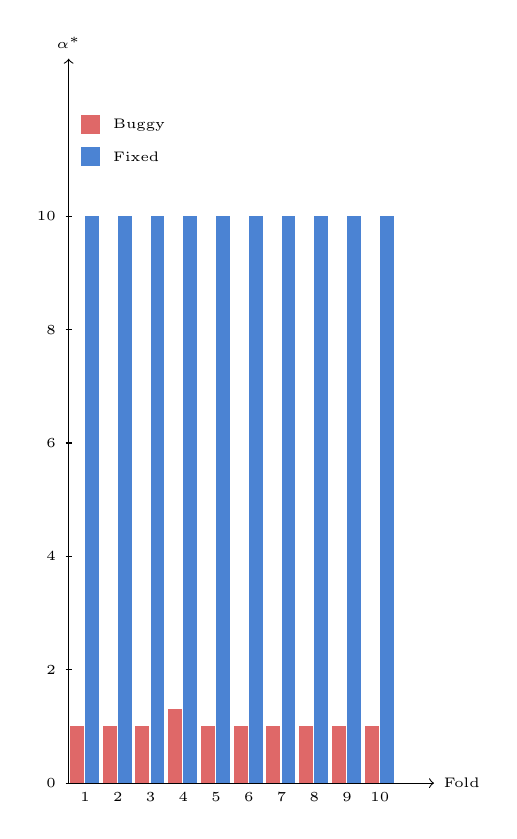
\begin{tikzpicture}[scale=0.80]
				\pgfmathsetmacro{\ymax}{11.5}
				% axes
				\draw[->] (0,0) -- (0,\ymax) node[above,font=\tiny]{$\alpha^*$};
				\draw[->] (0,0) -- (5.8,0) node[right,font=\tiny]{Fold};
				% y ticks
				\foreach \y in {0,2,4,6,8,10}{
					\draw (-0.05,\y*0.9) -- (0.05,\y*0.9);
					\node[left,font=\tiny] at (-0.05,\y*0.9) {\y};
				}
				% x ticks
				\foreach \i/\lbl in {1/1,2/2,3/3,4/4,5/5,6/6,7/7,8/8,9/9,10/10}{
					\pgfmathsetmacro{\xpos}{(\i-0.5)*0.52}
					\node[below,font=\tiny] at (\xpos,0) {\lbl};
				}
				% Buggy bars -- red (fold4=1.3, others=1.0)
				\foreach \i/\val in {1/1.0,2/1.0,3/1.0,4/1.3,5/1.0,6/1.0,7/1.0,8/1.0,9/1.0,10/1.0}{
					\pgfmathsetmacro{\xpos}{(\i-1)*0.52+0.02}
					\pgfmathsetmacro{\h}{\val*0.9}
					\fill[negred!70] (\xpos,0) rectangle ++(0.22,\h);
				}
				% Fixed bars -- all 10.0
				\foreach \i in {1,...,10}{
					\pgfmathsetmacro{\xpos}{(\i-1)*0.52+0.26}
					\fill[posblue!80] (\xpos,0) rectangle ++(0.22,9.0);
				}
				% legend
				\fill[negred!70] (0.2,10.3) rectangle ++(0.3,0.3);
				\node[right,font=\tiny] at (0.55,10.45) {Buggy};
				\fill[posblue!80] (0.2,9.8) rectangle ++(0.3,0.3);
				\node[right,font=\tiny] at (0.55,9.95) {Fixed};
			\end{tikzpicture}

			\vspace{0.3em}
			{\small\color{negred}$\Rightarrow$ 버그 버전: 유사도 범위 $[0.36,1]$로 압축 $\rightarrow$ $\alpha$ 변환 효과 미미 $\rightarrow$ $\alpha^*\approx 1.0$}\\[2pt]
			{\small\color{posblue}$\Rightarrow$ 수정 후: 유사도 범위 $[0,1]$ 정상화 $\rightarrow$ 모든 fold에서 $\alpha^*=10.0$ (탐색 상한 포화)}
	\end{columns}
\end{frame}

%─────────────────────────────────────────────────────────────────────────────
% α* Method × Fold 표 (4개): (K,TopN) = (10,5),(10,20),(20,5),(20,20)
% 주: α*는 TopN에 무관 → (10,5)=(10,20), (20,5)=(20,20) 동일
%─────────────────────────────────────────────────────────────────────────────

\begin{frame}[shrink=20]{$\lambda=0$\; $\alpha^*$ 선택: Method $\times$ Fold\quad $(K=10,\ \mathrm{TopN}=5)$}
	\framesubtitle{수정 후(Fixed)\quad {\color{negred}(괄호: 버기 값)}\quad {\color{posblue}★}: 수정된 메서드 (msd / jmsd / acos)}
	\centering
	\renewcommand{\arraystretch}{1.20}
	\small
	\begin{tabular}{@{}l@{\quad}c@{\quad}c@{\quad}c@{\quad}c@{\quad}c@{\quad}c@{\quad}c@{\quad}c@{\quad}c@{\quad}c@{}}
		\toprule
		Method & F01 & F02 & F03 & F04 & F05 & F06 & F07 & F08 & F09 & F10 \\
		\midrule
		\rowcolor{posblue!18}
		{\color{posblue}★}\,acos & .20\,{\color{negred}(7.00)} & .10\,{\color{negred}(6.50)} & .15\,{\color{negred}(6.50)} & .25\,{\color{negred}(7.00)} & .15\,{\color{negred}(7.00)} & .15\,{\color{negred}(7.00)} & .15\,{\color{negred}(6.50)} & .25\,{\color{negred}(6.50)} & .20\,{\color{negred}(7.00)} & .20\,{\color{negred}(7.00)} \\
		ami        & .05 & .05 & .05 & .05 & .05 & .05 & .05 & .05 & .05 & .05 \\
		ari        & .05 & .05 & .05 & .05 & .05 & .05 & .05 & .05 & .05 & .05 \\
		chebyshev  & .50 & .70 & .55 & .70 & .55 & .50 & .50 & .55 & .60 & .60 \\
		cosine     & 1.00 & 1.00 & .70 & 1.00 & 1.00 & 1.00 & 1.00 & 1.00 & 1.00 & 1.00 \\
		cpcc       & .85 & .65 & .55 & 1.00 & .50 & .70 & .60 & .60 & .35 & .65 \\
		euclidean  & .25 & .30 & .35 & .45 & .30 & .30 & .20 & .30 & .40 & .35 \\
		ipwr       & .95 & 1.00 & .80 & .95 & .85 & .95 & .90 & .85 & .75 & .80 \\
		itr        & .00 & .00 & .00 & .00 & .00 & .00 & .00 & .00 & .00 & .00 \\
		jaccard    & 1.00 & 1.00 & .65 & 1.00 & 1.00 & 1.00 & .80 & 1.00 & 1.00 & 1.00 \\
		\rowcolor{posblue!18}
		{\color{posblue}★}\,jmsd & 1.55\,{\color{negred}(1.40)} & 1.40\,{\color{negred}(1.30)} & .95\,{\color{negred}(.70)} & 1.25\,{\color{negred}(1.05)} & 1.35\,{\color{negred}(1.25)} & 1.45\,{\color{negred}(1.35)} & 1.10\,{\color{negred}(.90)} & 1.50\,{\color{negred}(1.35)} & .90\,{\color{negred}(.80)} & 1.10\,{\color{negred}(1.00)} \\
		kendall\_tau\_b & .10 & .05 & .05 & .30 & .05 & .20 & .15 & .25 & .10 & .25 \\
		manhattan  & .10 & .10 & .20 & .25 & .15 & .10 & .10 & .10 & .20 & .20 \\
		\rowcolor{posblue!18}
		{\color{posblue}★}\,msd  & 8.50\,{\color{negred}(10.0)} & 7.50\,{\color{negred}(10.0)} & 6.50\,{\color{negred}(10.0)} & 8.50\,{\color{negred}(10.0)} & 6.50\,{\color{negred}(10.0)} & 7.00\,{\color{negred}(10.0)} & 6.00\,{\color{negred}(10.0)} & 7.50\,{\color{negred}(10.0)} & 6.00\,{\color{negred}(9.50)} & 8.00\,{\color{negred}(10.0)} \\
		pcc        & .45 & .20 & .20 & .40 & .15 & .50 & .05 & .45 & .20 & .40 \\
		spcc       & .60 & .30 & .30 & .45 & .20 & .60 & .05 & .60 & .30 & .50 \\
		src        & .10 & .10 & .05 & .35 & .05 & .15 & .20 & .30 & .05 & .25 \\
		\bottomrule
	\end{tabular}

	\vspace{0.4em}
	\begin{beamercolorbox}[rounded=true,shadow=false,wd=\linewidth]{block body}
		\small 수정된 3개(★)만 Fixed↔Buggy 차이 발생. 나머지 14개는 Fixed=Buggy (유사도 미변경). $\alpha^*$는 TopN과 무관.\\
		버기 MSD: K=10에서 $\alpha^*\approx10$ (상한 고착, 버기 유사도 특성), 버기 JMSD: $\alpha^*=0.7\sim1.4$ (msd 버그 파급 확인).
	\end{beamercolorbox}
\end{frame}

\end{document}
